\section{Loudness}

%%%%%%%%%%%%%%%%%%%%%%%%%%%%%%%%%%%%%%%
\bi

\i Loudness is our perception of the relative 
strength of a sound.
It depends on the amplitude of the sound wave,
its frequency, and its duration.
(Here we will concentrate on the loudness of pure tones;
the perceived loudness of complex tones depends on the
frequency distribution of the sound.)
%broadband sounds (like white noise)
%are perceived to be louder than than equally intense
%pure tones.)

\i Loudness is a {\em relative} quantity in 
the sense that it involves a comparison between 
two different sounds---e.g., we say that this 
sound is twice as loud as that one.
In many of the formulae below, we will take our 
reference sound to be at the threshold of hearing.

\i As we shall describe in more detail below,
the human ear is most sensitive to sounds
with frequencies around 4000~Hz.
For example, a sound wave with a frequency of
100~Hz is perceived to be quieter than 
a sound wave with the same amplitude, 
but with a frequency of 4000~Hz.
%(See Figure~\ref{f:equal-loudness}.)

\i Sounds with durations less than about a half
a second are perceived to be quieter than the 
same sound having a duration of about a second.

\i The loudness of a sound that has 
a duration greater than several tens of seconds 
is perceived to {\em decrease} slightly over time.

\i This is due to {\em sensory adaptation} of
the brain.
A long-duration stimulus is increasingly ignored
by the brain as it realizes that there is no 
associated danger.
The firing rate of neurons decreases as the
duration of the stimulus increases;
the firing rate increases when there is a {\em change} 
in the stimulus.

\i Loudness depends on the {\em intensity} of
a sound wave but is not equal to it.
As we shall see below, loudness is more closely
related to the {\em logarithm} of the intensity, 
in line with Fechner's law relating stimulus 
to sensation.

\ei
%%%%%%%%%%%%%%%%%%%%%%%%%%%%%%%%%%%%%%%%%%%%%%
\subsection{Intensity, sound intensity level (W/m$^2$, dB)}
\bi

\i Recall that the intensity of a wave is the
rate at which energy passes through a unit area
perpendicular to the direction of wave propagation.
The units of intensity are W/m$^2$, corresponding 
to ${\rm energy}/({\rm area}\cdot{\rm time})$.

\i The intensity $I$ of a sound wave is related to 
the pressure deviation $p$ via
%
\be
I= \frac{p^2}{\rho v}
\label{e:Ivsrho2}
\ee
%
where $\rho$ is the density of air and $v$ is the speed 
of sound.
Thus, the intensity is proportional to the 
{\em squared amplitude} of the sound wave.

\i The {\em sound intensity level} SIL 
 is defined as
%
\be
{\rm SIL} = \log(I/I_0)\ {\rm bels}
= 10\log(I/I_0)\ {\rm dB}
\ee
%
where $I_0=10^{-12}~{\rm W}/{\rm m}^2$ is the intensity
for the threshold of hearing at $f=1000~{\rm Hz}$.

\i Note that 10~dB (decibels) equals 1 bel.
(A bel is named after Alexander Graham Bell, the inventor
of the telephone.)

\i \ex Doubling the intensity of a sound wave
corresponds to an increase in the sound intensity 
level by $10\log 2 \approx 3~{\rm dB}$.

\ex Increasing the intensity of a sound wave by
a factor of 10 corresponds to an increase in the 
sound intensity level by $10\log 10 = 10~{\rm dB}$.

\i The {\em just noticeable difference} (JND) for 
intensity is about 1~dB.
This is the increase in sound intensity level
needed in order for the change in sound intensity 
(for two notes played sequentially) to be just noticeable.

\i In terms of a percent, a 1~dB increase in 
SIL corresponds to a 26\% increase in intensity since
%
\be
10^{1/10} = 1.26
\ee

\ei
%%%%%%%%%%%%%%%%%%%%%%%%%%%%%%%%%%%%%%%%%%%%%%%%%
\subsection{Sound loudness level (phon)}
\bi

\i Although sound intensity level SIL is a 
quantative measure of the strength of a sound wave,
it doesn't take into account the frequency-dependence
of the response of the human ear.

\i In 1933, H.~Fletcher and W.A.~Munson experimentally 
determined {\em equal-loudness} curves for pure 
tones by carrying out tests on many people.
Their results were very similar to those shown
in Figure~\ref{f:equal-loudness}, which have been
recommended by the International Standards Organization.
%
\begin{figure}[htbp]
\begin{center}
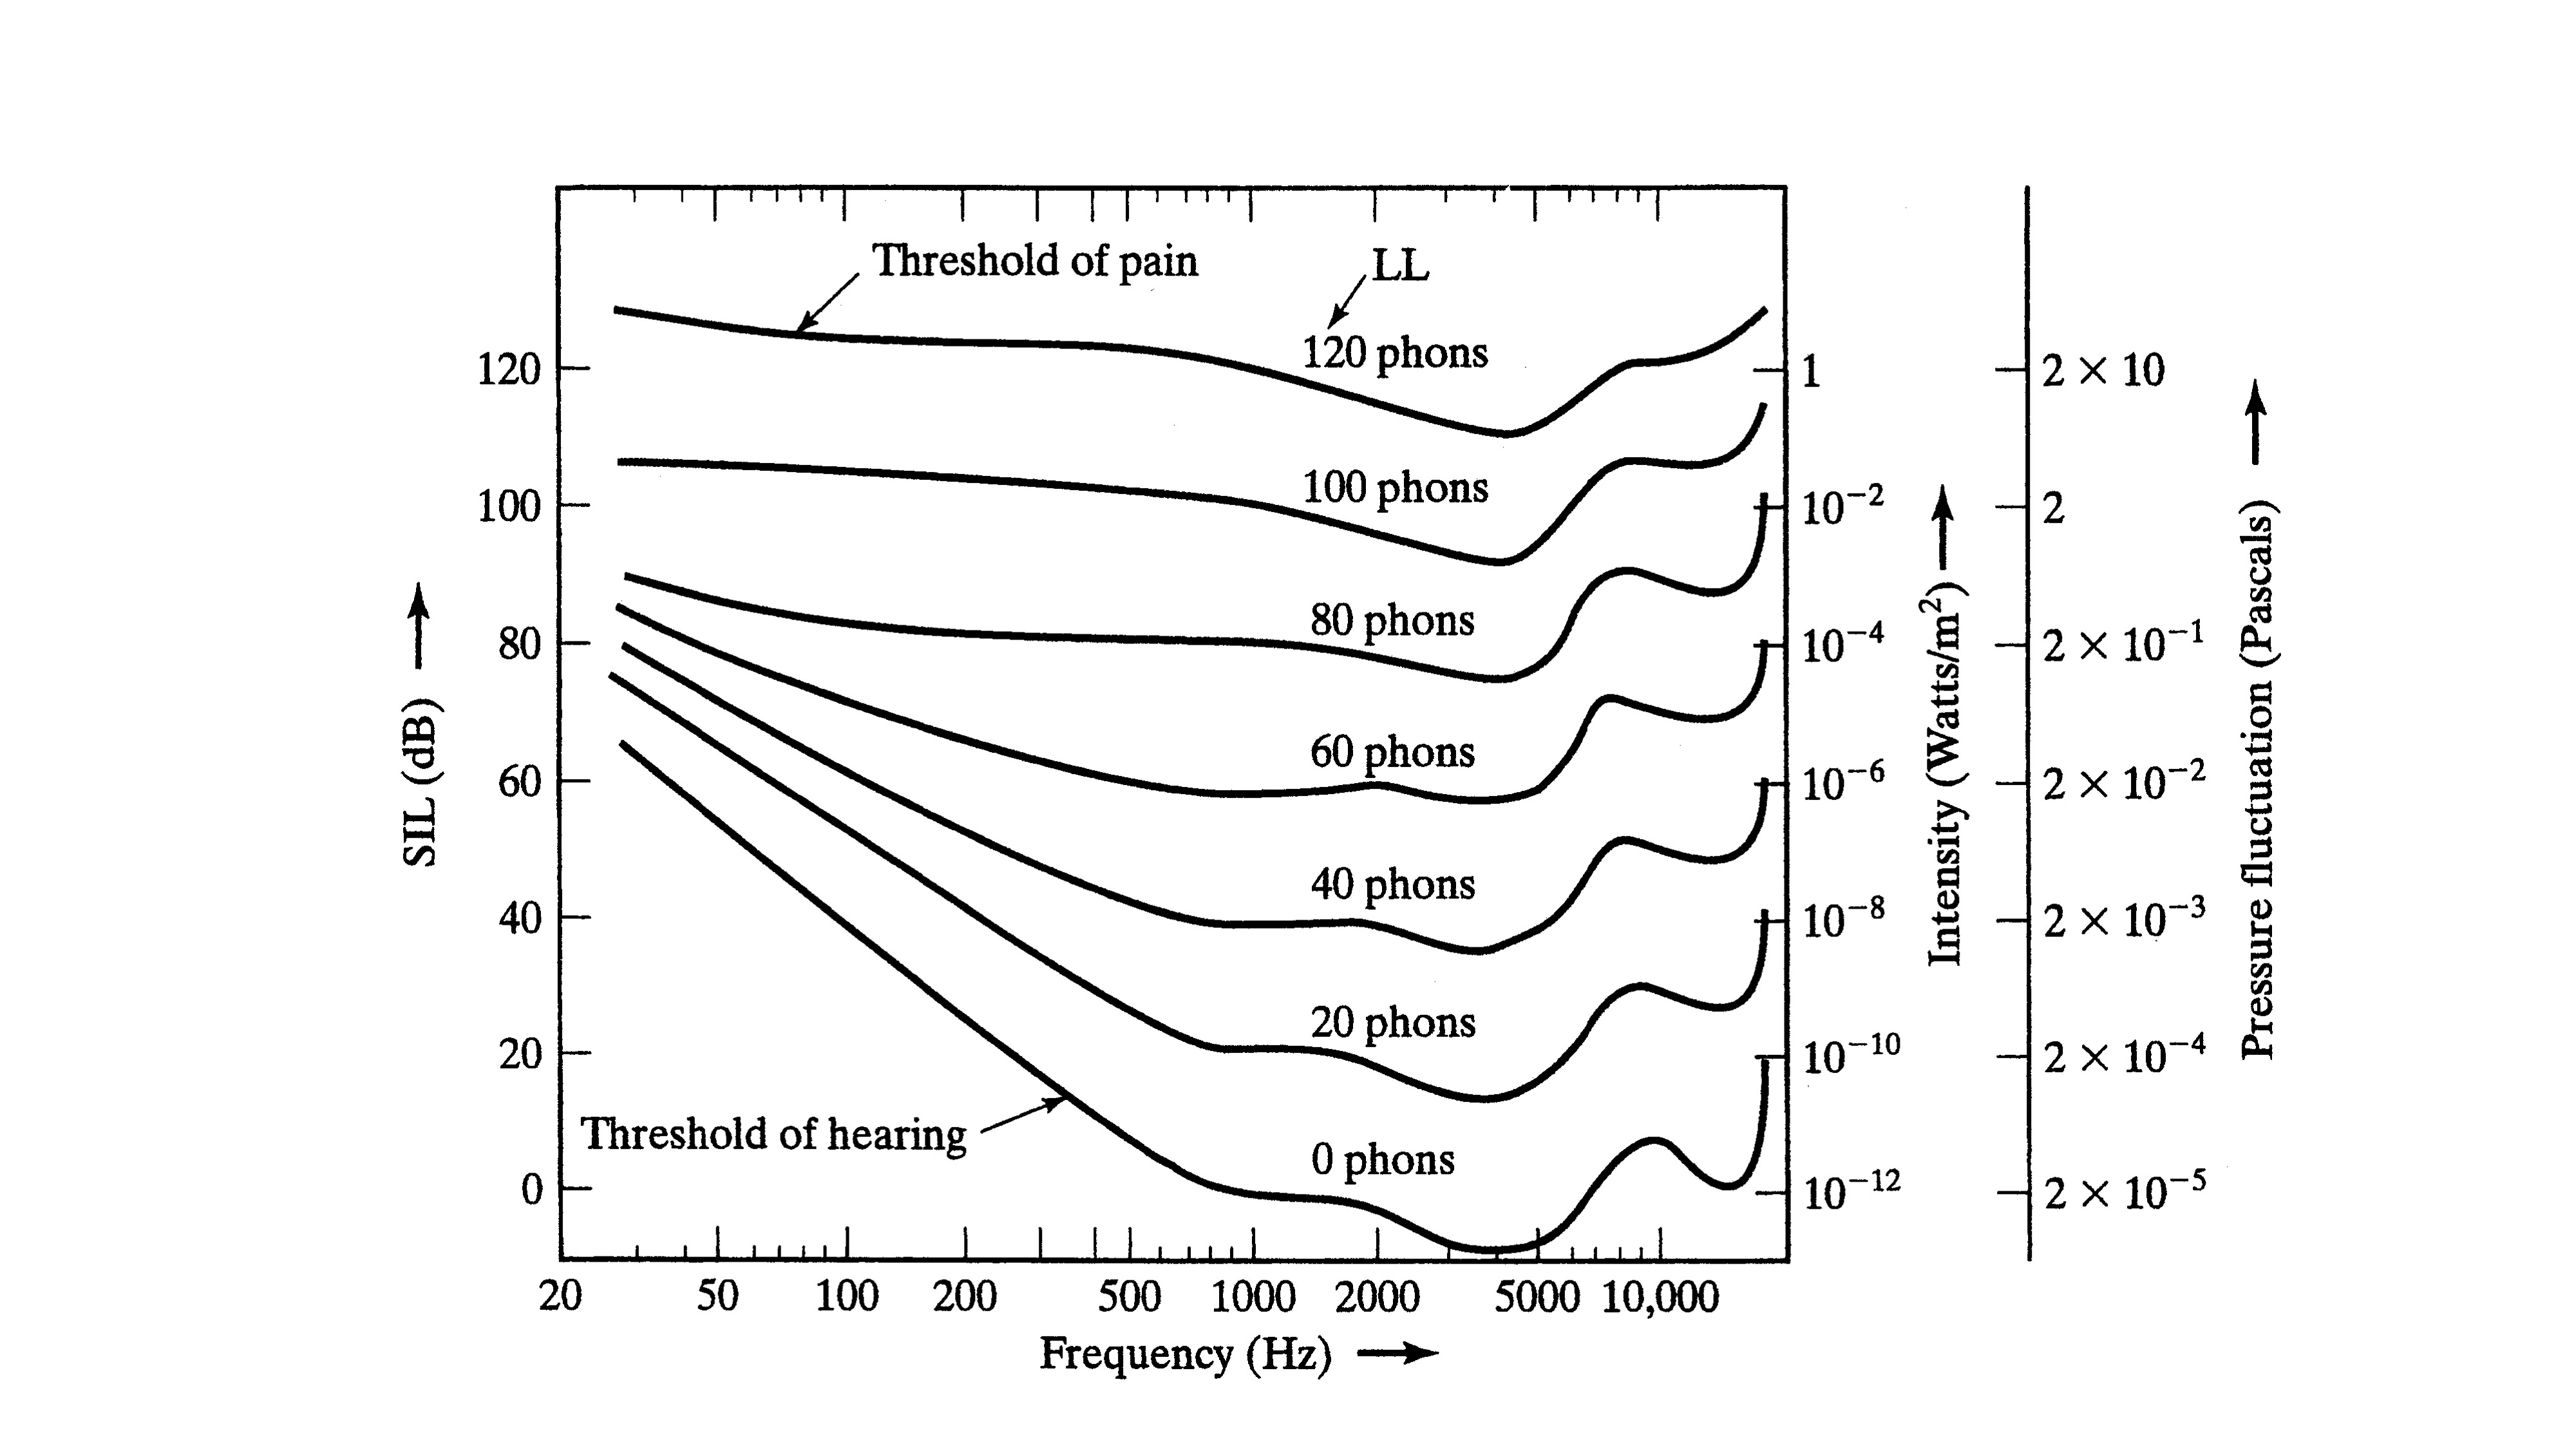
\includegraphics[width=0.8\textwidth]{fletcher-munson}
\caption{Equal-loudness curves (labeled in units of phons) 
for the human ear.
Note that the ear is most sensitive to frequencies around 4000~Hz.
(From ``Physics of Sound" by Berg and Stork.)}
\label{f:equal-loudness}
\end{center}
\end{figure}
%

\i The equal-loudness curves are labeled by values of
constant {\em sound loudness level} $L_L$.
The units of $L_L$ are {\em phons}.
Numerically, 
%
\be
L_L\ ({\rm phon}) = {\rm SIL}\ ({\rm dB})
\quad
{\rm at}\  f=1000~{\rm Hz}
\ee
%
In general, the value of $L_L$ depends on both SIL 
and the frequency $f$.

\i Curves of constant phon are perceived to be 
equally-loud at different frequencies.
This means that at low frequencies (e.g., 100~Hz), 
the sound pressure
level must be substantially higher than at 
$f=1000~{\rm Hz}$ for a sound to be perceived as being
equally loud.
From the figure, we see that our ears are most sensitive 
to sounds having frequencies near $f=4000~{\rm Hz}$.

\i \exer 
What is the sound intensity level at 100~Hz for a 
sound with a sound loudness level of 40~phon?

\i \ans 
Using Figure~\ref{f:equal-loudness}, we see that
the $L_L=40~{\rm phon}$ equal-loudness curve has
${\rm SIL}=60~{\rm dB}$ at $f=100~{\rm Hz}$.

\i A standard sound-level meter measures the sound 
intensity level with different frequency responses:
(i) C-weighting has a flat frequency response, 
corresponding to a measurement of SIL in dB;
(ii) A-weighting has a frequency response that mimics
the sensitivity of the human ear, corresponding to a
measurement of $L_L$ in phon (sometimes denoted dBA).

\ei
%%%%%%%%%%%%%%%%%%%%%%%%%%%%%%%%%%%%%%%%%%%%%%%%%
\subsection{Subjective loudness (sone)}
\bi

\i If the sound loudness level $L_L$ of one sound is 
10~phon larger than another sound, then most people 
perceive the first sound {\em to be twice as loud} as 
the second sound.  
(This corresponds to $\Delta{\rm SIL}=10~{\rm dB}$ 
or a factor of 10 increase in intensity at a frequency
of 1000~Hz.)

\i To quantify this ``twice as loud" dependence, one 
defines {\em subjective loudness} $S$ via
%
\be
S= \, 2^{(L_L-40)/10}~{\rm sone}
\ee
%
so that $S=1~{\rm sone}$ is equivalent to $L_L=40~{\rm phon}$,
and $S$ increases by a factor of 2 whenever $L_L$ increases
by 10~phon.

\i Table~\ref{t:loudnesslevels} compares different 
measures of loudness.
%
\begin{table}[htbp]
\begin{center}
\begin{tabular}{|c|c|c|c|}
\hline
& ${\rm SIL}$ (dB) at 1000 Hz & $L_L$ (phon) & $S$ (sone) \\
\hline
Threshold of hearing & 0 & 0 & 1/16 \\
Recording studio & 20 & 20 & 1/4 \\
Quiet office & 40 & 40 & 1 \\
Ordinary conversation & 60 & 60 & 4 \\
Normal piano practice & 80 & 80 & 16 \\
Piano fortissimo & 100 & 100 & 64 \\
Threshold of pain & 120 & 120 & 256 \\
\hline
\end{tabular}
\caption{Comparison of different measures of loudness.}
\label{t:loudnesslevels}
\end{center}
\end{table}

\i Figure~\ref{f:OSHA-table} is a table with the
Occupational Safety and Health Administration 
(OSHA) guidelines for noise exposure.
%
\begin{figure}[htbp]
\begin{center}
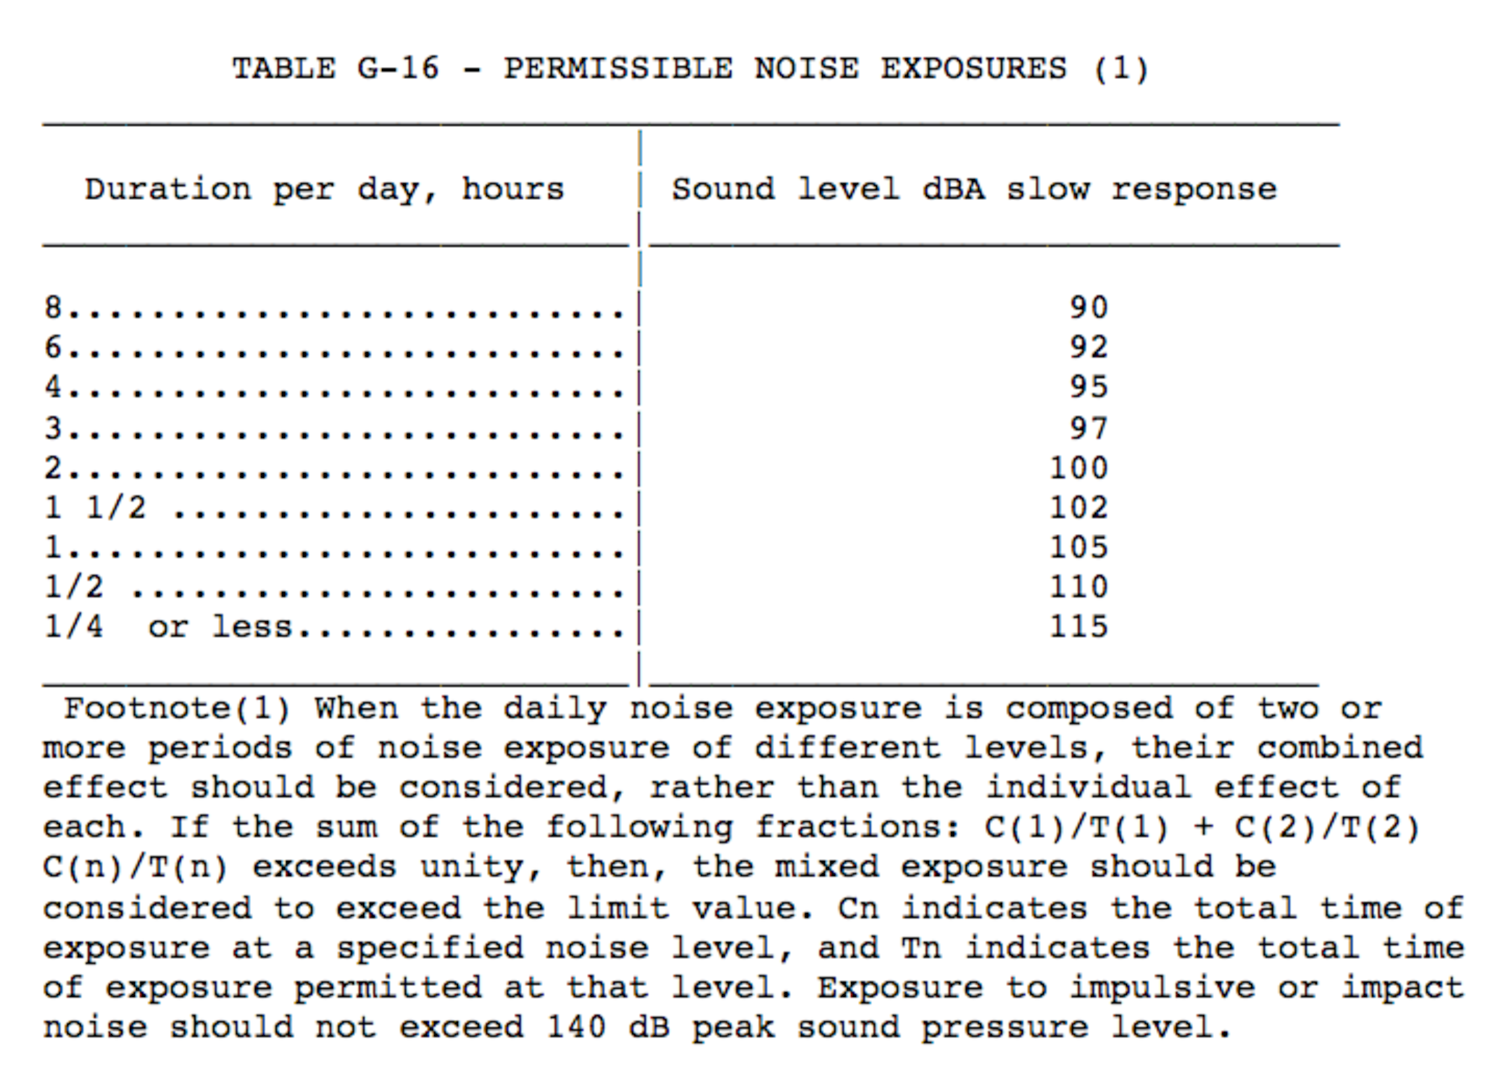
\includegraphics[width=0.8\textwidth]{OSHA-table}
\caption{OSHA permissible noise exposure levels.
(From {\tt www.osha.gov}, Standard Number: 1910.95.)}
\label{f:OSHA-table}
\end{center}
\end{figure}
%

\i The range of sound level in a musical 
performance is called its {\em dynamic range}.

\i The dynamic range of a performance 
is typically between 10-20~dB, 
although it may as high as 40~dB.
(Remember that a 10~dB increase in SIL at 1000~Hz
corresponds to a $2\times$ increase in perceived loudness.)

\ei
%%%%%%%%%%%%%%%%%%%%%%%%%%%%%%%%%%%%%%%%%%
\subsection{Sound from multiple sources}
\bi

\i Consider two instruments playing a note 
at the same time.
The sound waves from each instrument combine
with one another to produce a resultant wave 
with amplitude $p_{\rm tot}$ that can have 
any value between $p_1+p_2$ and $|p_1-p_2|$,
which depends on the phase relation of the waves,
where $p_1$, $p_2$ are the pressure amplitudes for
the two component waves.

\i On average, for random phases, the resultant 
amplitude will have a value
%
\be
p_{\rm tot} = \sqrt{p_1^2 + p_2^2}
\ee
%
This is called an {\em incoherent} superposition
of two waves.

\i Since intensity is proportional to the
square of the pressure amplitude, it follows that the
intensity of the incoherent sum of the two sound waves
is given, on average, by
%
\be
I_{\rm tot} = I_1+I_2
\ee
%
Thus, {\em intensities add}.

\i Hence, 2 violins playing simultaneously produce
an intensity $2\times$ greater than that of a single
violin; 10 violins playing simultaneously produce
an intensity $10\times$ greater.
The corresponding increase in the sound intensity 
level SIL will be
%
\begin{align}
&10\log 2 \approx 3~{\rm dB}\quad({\rm two\ violins})
\\
&10\log 10 = 10~{\rm dB}\quad({\rm ten\ violins})
\end{align}
%

\i Note that to double the subjective loudness level $S$ 
requires $L_L$ to increase by 10~phon 
(or ${\rm SIL}$ to increase by 10~dB at 1000~Hz).
This corresponds to a $10\times$ increase in the intensity $I$ 
of the sound at 1000~Hz.
{\em Hence, we would need 10~violins playing 
simultaneously to sound twice as loud as a single violin.}

\ei
